\section{Gesamtübersicht}
\begin{figure}[H]
\centering
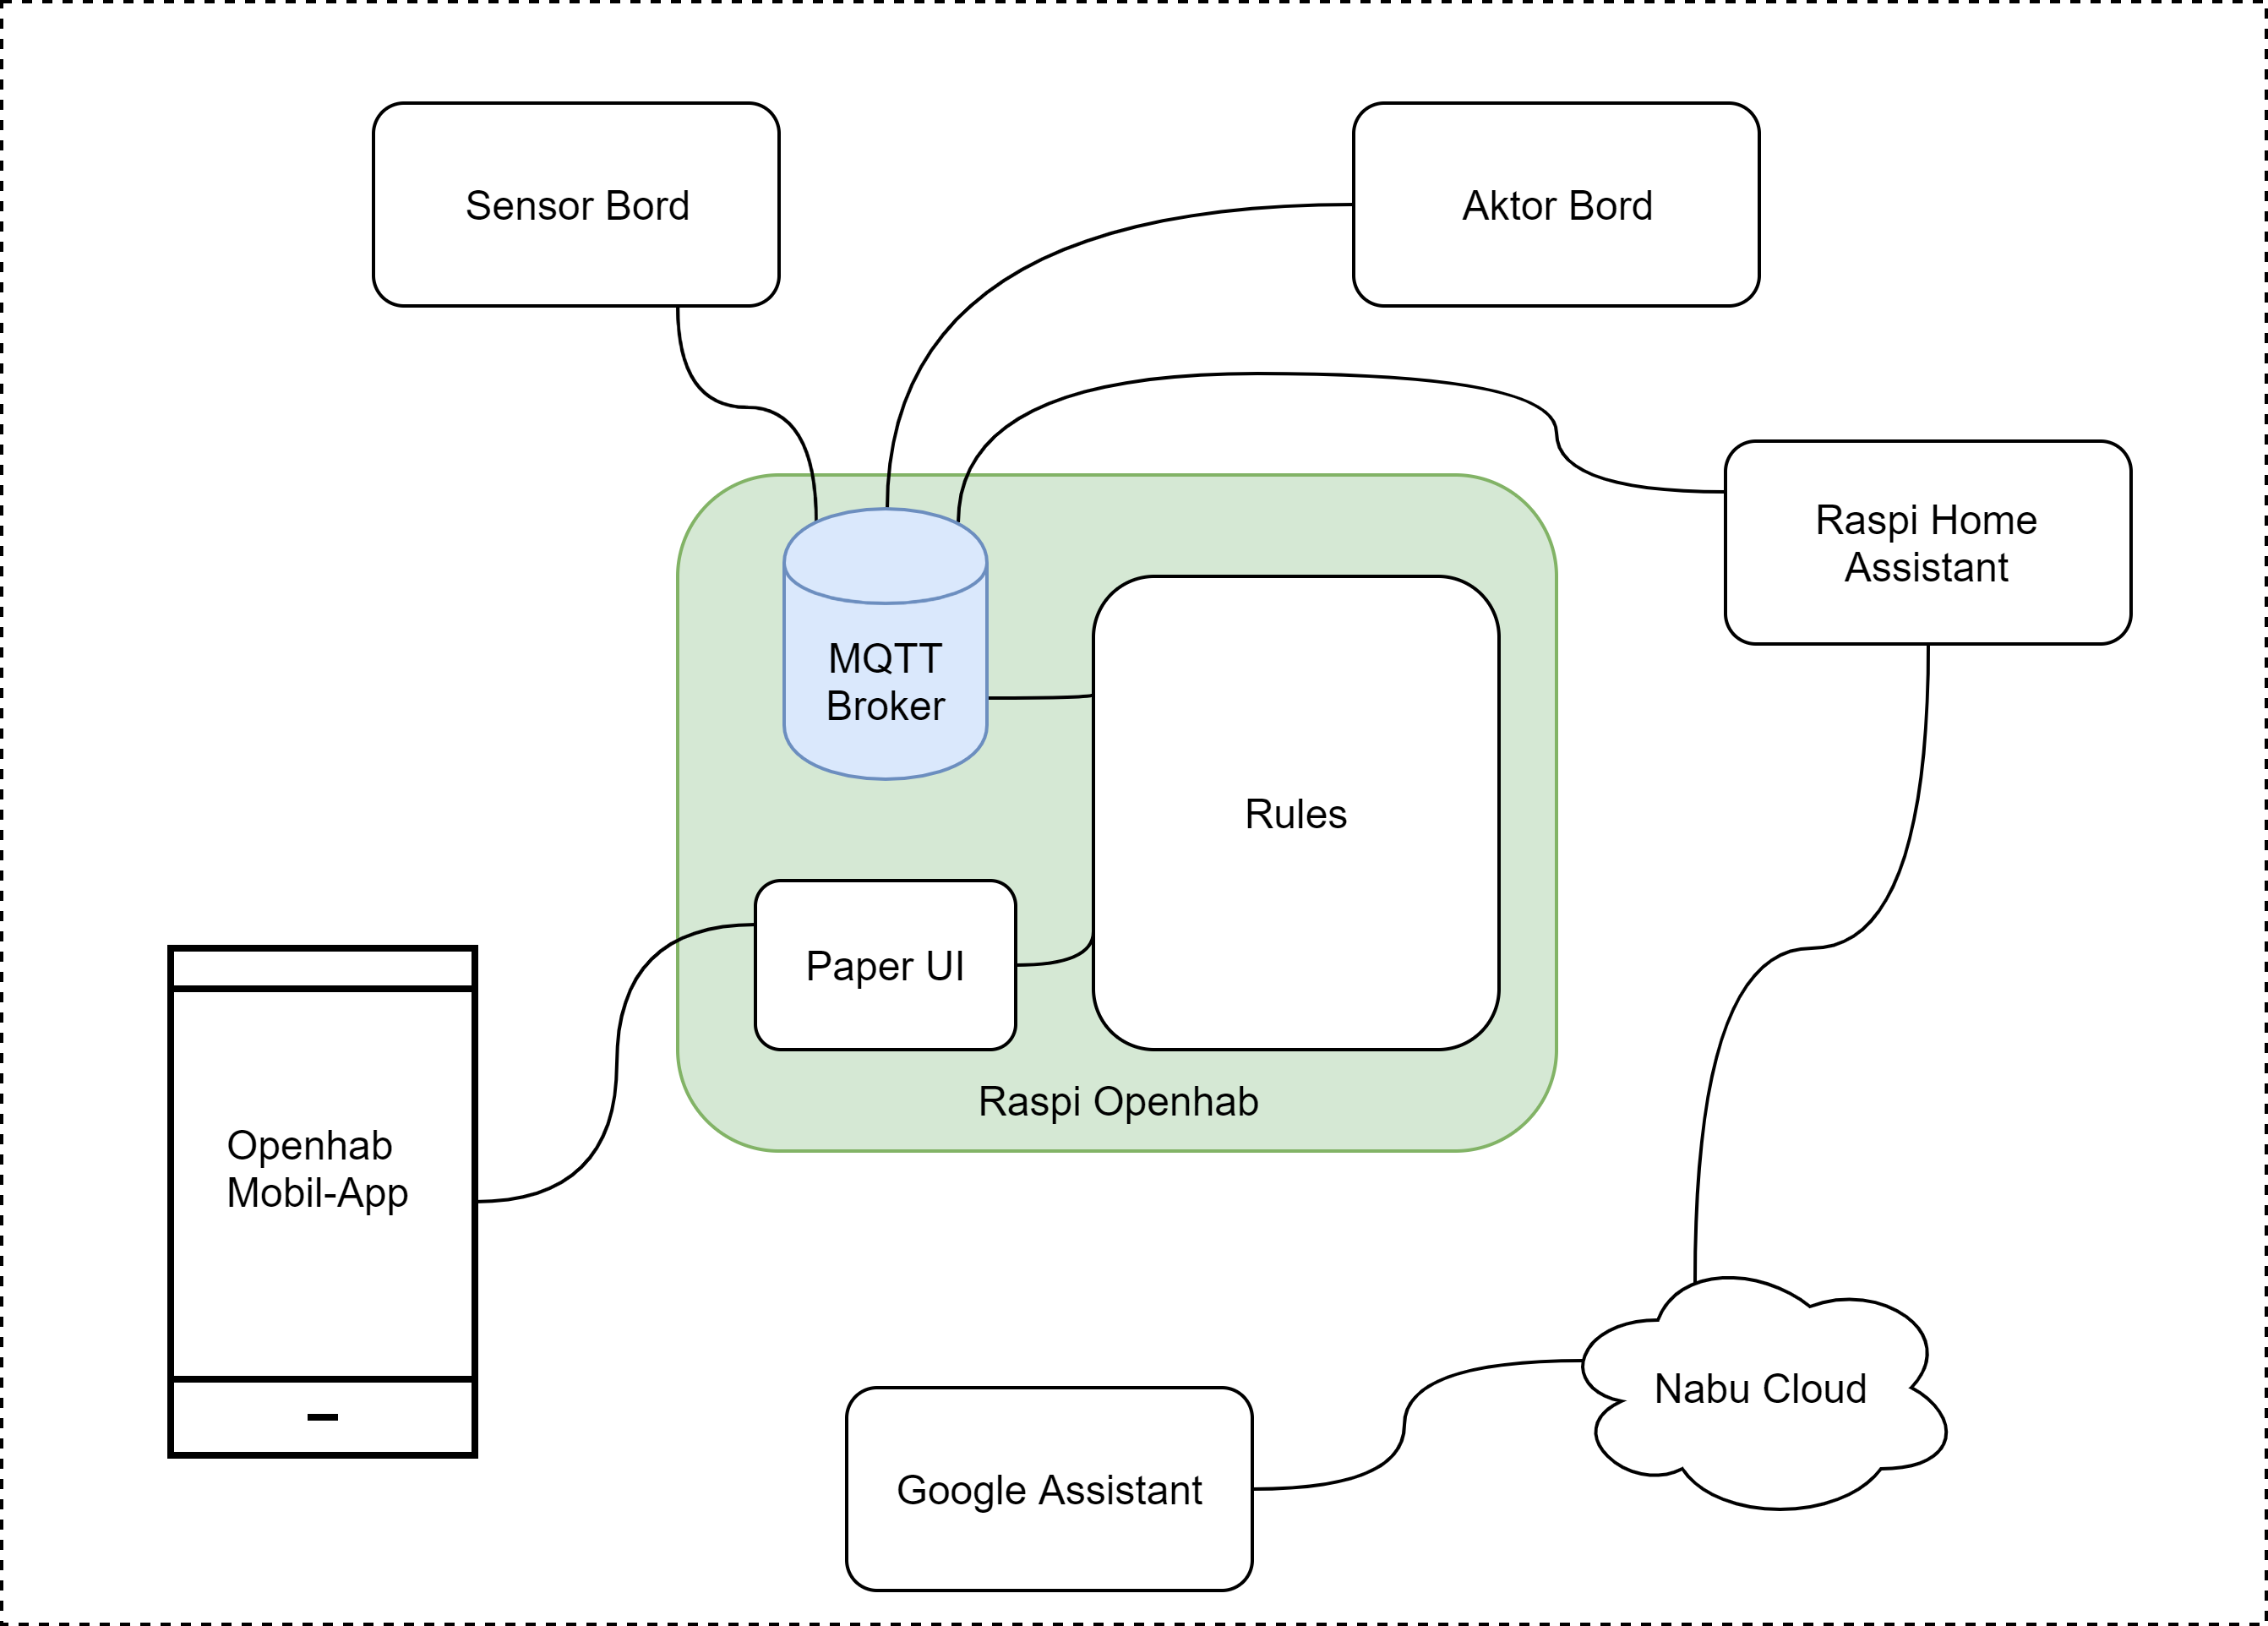
\includegraphics[width=\linewidth]{Gesammtubersicht.png}
\caption{Gesamtübersicht Komponenten Becholour Thesiss }
\label{pic: Gesamtübersicht}
\end{figure}
In der Abbildung \ref{pic: Gesamtübersicht} sind die Geräte und Ihre Verbindungen schematisch abgebildet. Als Herzstück dient der Openhab Server, welcher auf ein Rasperrypi aufgesetzt wurde. Ein eigener Mqtt-Broker, welcher die kommunikations-Messages managt wurde eingebunden. Verschiedene Geräte wie das Aktor- und Sensor Bord, auch der Home Assistant, welcher als Brücke für den Google Assistant dient, gelingt es im eigenen Lokalen Netzwerk zu kommunizieren. Als Web-Interface steht das Paper UI von Openhab wie auch das Mobile-App dem Benutzer, zum Bedienen vom System zur Verfügung. Mit den Rules sind alle Automatisierten Vorgänge in Openhab festgelegt, in diesem Projekt sind dies die Definitionen welchem Befehl welche Schalthandlungen durchgeführt werden müssen. Der Grund warum die Schalthandlungen und die Verknüpfungen in den Ruls definiert werden, liegt daran, dass so keine Programmiereingriffe in die Einzelnen Aktor- oder Sensor Bords Durchgeführt werden müssen. Der Benutzer kann die Konfigurationen in Openhab Graphisch im Web-Interface oder als Programmiercode in einem Editor wie Visual Studio Code durchführen, sieh Benutzerhandbuch Anhang.    




